\chapter{Nociones de álgebra lineal}\label{cap:algebra-lineal}

Muchos de los conceptos que utilizaremos en esta materia provienen del álgebra
lineal básica. Este capítulo tiene tres objetivos. El primero es repasar, sin
detenernos demasiado, las nociones que vamos a necesitar; el segundo es fijar la
notación y el vocabulario que usaremos en todo el apunte; y el tercero, que es
el más importante, es cambiar la forma de mirar una matriz. Al final del
capítulo una matriz habrá dejado de ser una tabla de números para pasar a ser un
objeto con \emph{cuatro subespacios} asociados y una primera factorización,
$A=CR$, que ya contiene casi toda la información que nos interesa.

\medskip

\noindent\textbf{Convenio.} Salvo aviso explícito, todos los escalares son
reales. El caso complejo aparecerá cuando lo necesitemos (Capítulos
\ref{cap:ortogonalidad} y siguientes) y avisaremos en cada caso.

\medskip

\noindent\textbf{Sobre los ejercicios de desarrollo.} A lo largo del apunte
aparecen, dentro del texto, algunos recuadros titulados \emph{Ejercicio de
desarrollo}. No son ejercicios de práctica: son partes de la teoría cuya
demostración queda a cargo del lector y que después usaremos con toda
naturalidad. Se entregan por escrito.

\section{Espacios vectoriales y subespacios}
\label{sec:espacios_vectoriales}

Un \textbf{espacio vectorial} sobre un cuerpo $\mathbb{F}$ (para nosotros,
$\mathbb{R}$ o $\mathbb{C}$) es un conjunto $V$ cuyos elementos llamamos
\textbf{vectores}, en el que están definidas una suma y un producto por
escalares que se comportan como uno espera: la suma es asociativa y conmutativa,
tiene un neutro $\n{0}$ y cada vector tiene su opuesto; el producto por
escalares es asociativo, tiene al $1$ como neutro y se distribuye respecto de
ambas sumas. No vamos a usar estos axiomas directamente casi nunca: los
necesitamos sólo para saber que tiene sentido hablar de combinaciones lineales.

Los espacios que efectivamente aparecerán en este curso son cuatro:
\begin{itemize}[itemsep=1pt]
\item $\mathbb{R}^n$ y $\mathbb{C}^n$, los vectores columna de $n$ componentes;
\item $\mathbb{R}^{m\times n}$, las matrices de $m$ filas y $n$ columnas;
\item $\mathcal{P}_n$, los polinomios de grado menor o igual que $n$;
\item los subespacios de los anteriores, que son el objeto central del capítulo.
\end{itemize}

\subsection{Subespacios}

Un subconjunto $S\subseteq V$ es un \textbf{subespacio} de $V$ si
\begin{enumerate}[itemsep=1pt,label=(\roman*)]
    \item $\n{0}\in S$;
    \item $\n{x},\n{y}\in S\implies \n{x}+\n{y}\in S$;
    \item $\n{x}\in S$, $\alpha\in\mathbb{F}\implies \alpha\n{x}\in S$.
\end{enumerate}
Las condiciones (ii) y (iii) dicen que $S$ es \emph{cerrado} por las dos
operaciones; junto con (i) garantizan que $S$, con las operaciones heredadas, es
él mismo un espacio vectorial. Los ejemplos triviales son $\{\n{0}\}$ y el
propio $V$.

Sean $U$ y $W$ subespacios de $V$. La \textbf{suma}
\[
U + W = \{\n{u} + \n{w} : \n{u} \in U,\ \n{w} \in W\}
\]
y la \textbf{intersección} $U\cap W$ son también subespacios de $V$: la primera
es el subespacio más chico que contiene a $U$ y a $W$, y la segunda el más
grande contenido en ambos. Si además $U \cap W = \{\n{0}\}$, la suma se llama
\textbf{suma directa} y se escribe $U \oplus W$; en ese caso cada vector de
$U+W$ se escribe de manera \textbf{única} como $\n{u} + \n{w}$ con $\n{u} \in U$
y $\n{w} \in W$.

\subsection{Combinaciones lineales, independencia y bases}

Dados $\n{v}_1, \dots, \n{v}_k \in V$ y escalares $\alpha_1, \dots, \alpha_k$,
la expresión $\alpha_1 \n{v}_1 + \cdots + \alpha_k \n{v}_k$ es una
\textbf{combinación lineal} de los $\n{v}_i$.

El conjunto $\{\n{v}_1, \dots, \n{v}_k\}$ es \textbf{linealmente independiente}
si la única combinación lineal que da el vector nulo es la trivial:
\[
\sum_{i=1}^k \alpha_i \n{v}_i = \n{0}
\quad \Longrightarrow \quad \alpha_i = 0 \ \text{ para todo } i.
\]
Si no, los vectores son \textbf{linealmente dependientes}, y entonces al menos
uno de ellos es combinación lineal de los demás.

El conjunto de \emph{todas} las combinaciones lineales de
$S = \{\n{u}_1, \dots, \n{u}_k\}$ es un subespacio de $V$, el \textbf{subespacio
generado} por $S$:
\[
\gen(S) = \Big\{ \sum_{i=1}^k \alpha_i \n{u}_i \ :\ \alpha_i \in \mathbb{F} \Big\}.
\]

Una \textbf{base} de $V$ es un conjunto linealmente independiente que genera
$V$. Si $B = \{\n{v}_1, \dots, \n{v}_n\}$ es una base, todo $\n{v} \in V$ se
escribe de manera \textbf{única} como $\n{v} = \alpha_1 \n{v}_1 + \cdots +
\alpha_n \n{v}_n$, y los escalares $\alpha_i$ se llaman \textbf{coordenadas} de
$\n{v}$ en la base $B$. Todas las bases de $V$ tienen la misma cantidad de
elementos; ese número es la \textbf{dimensión} $\dim(V)$. Por ejemplo
$\dim \mathbb{R}^n = n$, con la base canónica
\[
\n{e}_1 = (1,0,\dots,0)^T, \quad
\n{e}_2 = (0,1,\dots,0)^T, \quad \dots, \quad
\n{e}_n = (0,0,\dots,1)^T .
\]

\section{Transformaciones lineales y matrices}

Sean $V$ y $W$ espacios vectoriales sobre el mismo cuerpo. Una función
$T: V \to W$ es una \textbf{transformación lineal} si respeta las dos
operaciones:
\[
T(\n{u} + \n{v}) = T(\n{u}) + T(\n{v}),
\qquad
T(\alpha \n{v}) = \alpha\, T(\n{v}),
\]
o, equivalentemente, si ``entra'' por las combinaciones lineales:
$T\big(\sum_i \alpha_i \n{v}_i\big) = \sum_i \alpha_i T(\n{v}_i)$.

En $\mathbb{R}^2$ son lineales la homotecia $T(x,y) = (2x, 2y)$ y la reflexión
$T(x,y) = (x, -y)$; en $\mathcal{P}_n(\mathbb{R})$ lo es la derivación
$D(p) = p'$. No es lineal $T(x,y) = (x+1, y)$, porque $T(\n{0}) = (1,0) \neq
\n{0}$: toda transformación lineal manda el cero al cero.

Dos subespacios acompañan a cada transformación lineal: el \textbf{núcleo}
\[
\ker(T) = \{\n{v} \in V : T(\n{v}) = \n{0}_W\} \subseteq V
\]
y la \textbf{imagen}
\[
\im(T) = \{T(\n{v}) : \n{v} \in V\} \subseteq W .
\]
Por ejemplo, para $T:\mathbb{R}^3 \to \mathbb{R}^2$ con $T(x,y,z) = (x,y)$, el
núcleo es el eje $z$ y la imagen es todo $\mathbb{R}^2$.

\subsection{De la transformación a la matriz}

Como $T$ es lineal, queda completamente determinada por lo que les hace a los
vectores de una base: si sabemos calcular $T(\n{v}_1),\dots,T(\n{v}_n)$, sabemos
calcular $T$ en cualquier vector. Esto es lo que permite reemplazar a $T$ por una
tabla de números.

Concretamente, tomemos $T:\mathbb{R}^n\to\mathbb{R}^m$ y las bases canónicas.
La \textbf{matriz de $T$} es la matriz $A\in\mathbb{R}^{m\times n}$ cuya columna
$j$ es el vector $T(\n{e}_j)$:
\[
A = \begin{bmatrix} T(\n{e}_1) & T(\n{e}_2) & \cdots & T(\n{e}_n)\end{bmatrix},
\qquad\text{y entonces}\qquad
T(\n{x}) = A\n{x} \ \text{ para todo } \n{x}\in\mathbb{R}^n .
\]

\begin{example}
Sea $T(x_1, x_2) = (x_1 + x_2,\, 2x_1,\, x_1 - x_2)$. Como $T(1,0) = (1,2,1)$ y
$T(0,1) = (1,0,-1)$,
\[
A = \begin{bmatrix} 1 & 1 \\ 2 & 0 \\ 1 & -1 \end{bmatrix}
\qquad\text{y en efecto}\qquad
A \begin{bmatrix} a \\ b \end{bmatrix}
= \begin{bmatrix} a + b \\ 2a \\ a - b \end{bmatrix} = T(a,b).
\]
\end{example}

\begin{remark}[Otras bases]\label{obs:otras-bases}
Nada obliga a usar las bases canónicas. Si $B_V$ y $B_W$ son bases cualesquiera
de $V$ y $W$, la columna $j$ de la matriz de $T$ es el vector de coordenadas de
$T(\n{v}_j)$ en la base $B_W$, y el producto matriz por vector sigue calculando
las coordenadas de la imagen. Cambiar de base cambia la matriz pero no la
transformación: dos matrices que representan la misma transformación en bases
distintas se llaman \emph{semejantes}, y las estudiaremos en el
Capítulo~\ref{cap:autovalores}. Hasta entonces trabajaremos siempre con las
bases canónicas de $\mathbb{R}^n$ y $\mathbb{R}^m$, de modo que
\emph{transformación lineal} y \emph{matriz} serán sinónimos.
\end{remark}

Por último, la composición de transformaciones lineales corresponde al
\textbf{producto} de matrices: si $T$ tiene matriz $A$ y $S$ tiene matriz $B$
(con las dimensiones compatibles), entonces $S\circ T$ tiene matriz $BA$. Esta
es la verdadera razón de ser de la regla de multiplicación de matrices, que
revisaremos en detalle en la Sección~\ref{sec:producto}.

\section{Matrices: operaciones y vocabulario}
\label{sec:vocabulario}

\subsection{El espacio vectorial $\mathbb{R}^{m\times n}$}

Una \textbf{matriz} es un arreglo rectangular de $m$ filas y $n$ columnas,
\[
A =
\begin{bmatrix}
a_{11} & a_{12} & \cdots & a_{1n} \\
a_{21} & a_{22} & \cdots & a_{2n} \\
\vdots & \vdots & \ddots & \vdots \\
a_{m1} & a_{m2} & \cdots & a_{mn}
\end{bmatrix} \in \mathbb{R}^{m \times n},
\]
y escribimos $(A)_{ij} = a_{ij}$. Notaremos
\[
\fila_i(A) = \begin{bmatrix} a_{i1} & a_{i2} & \cdots & a_{in}\end{bmatrix}
\in\mathbb{R}^{1\times n},
\qquad
\col_j(A) = \begin{bmatrix} a_{1j} \\ a_{2j} \\ \vdots \\ a_{mj}\end{bmatrix}
\in\mathbb{R}^{m}.
\]
Con la suma y el producto por escalares definidos entrada a entrada,
$(A+B)_{ij} = a_{ij}+b_{ij}$ y $(\alpha A)_{ij} = \alpha a_{ij}$, el conjunto
$\mathbb{R}^{m\times n}$ es un espacio vectorial de dimensión $mn$.

\subsection{Traspuesta}

La \textbf{traspuesta} de $A\in\mathbb{R}^{m\times n}$ es la matriz
$A^T\in\mathbb{R}^{n\times m}$ dada por $(A^T)_{ij} = a_{ji}$: las filas de $A$
son las columnas de $A^T$. Valen
\[
(A^T)^T = A,
\qquad
(A+B)^T = A^T+B^T,
\qquad
\boxed{\,(AB)^T = B^T A^T\,},
\]
y la última, que invierte el orden, se usará constantemente. Una matriz cuadrada
es \textbf{simétrica} si $A^T = A$. Para cualquier $A\in\mathbb{R}^{m\times n}$,
las matrices $A^TA\in\mathbb{R}^{n\times n}$ y $AA^T\in\mathbb{R}^{m\times m}$
son simétricas; volverán a aparecer en proyecciones, en cuadrados mínimos y en
la SVD.

\subsection{Matrices con nombre propio}

\begin{itemize}[itemsep=2pt]
\item La \textbf{identidad} $I_n\in\mathbb{R}^{n\times n}$ tiene unos en la
diagonal y ceros fuera; sus columnas son $\n{e}_1,\dots,\n{e}_n$ y cumple
$AI = A$, $IA = A$.
\item $A$ cuadrada es \textbf{invertible} (o no singular) si existe $A^{-1}$ con
$AA^{-1} = A^{-1}A = I$. La inversa, cuando existe, es única, y
$(AB)^{-1} = B^{-1}A^{-1}$, $(A^{-1})^T = (A^T)^{-1}$.
\item $D = \diag(d_1,\dots,d_n)$ es \textbf{diagonal} si $d_{ij} = 0$ para
$i \neq j$. Multiplicar $DA$ escala las \emph{filas} de $A$ y $AD$ escala las
\emph{columnas}.
\item $A$ es \textbf{triangular superior} si $a_{ij} = 0$ para $i > j$, e
\textbf{inferior} si $a_{ij} = 0$ para $i < j$. Son las protagonistas del
Capítulo~\ref{cap:LU}.
\item Una matriz de \textbf{permutación} $P$ tiene exactamente un $1$ en cada
fila y en cada columna y ceros en el resto; $PA$ permuta las filas de $A$ y
$P^{-1} = P^T$.
\end{itemize}

\subsection{Traza}

La \textbf{traza} de una matriz cuadrada es la suma de su diagonal,
\[
\tr(A) = \sum_{i=1}^n a_{ii}.
\]
Es lineal, $\tr(A^T) = \tr(A)$, y cumple la identidad
$\tr(AB) = \tr(BA)$ cada vez que ambos productos tienen sentido (Ejercicio
\ref{ej:traza}), aunque $AB \neq BA$. La traza reaparecerá como suma de
autovalores, como rango de una proyección y dentro de la norma de Frobenius.

\subsection{El producto escalar y la norma euclídea}
\label{sec:producto-escalar}

Antes de seguir conviene fijar las dos operaciones con las que se mide en
$\mathbb{R}^n$, que usaremos desde acá en adelante. Dados
$\n{x}=(x_1,\dots,x_n)^T$ e $\n{y}=(y_1,\dots,y_n)^T$, el \textbf{producto
escalar} (o producto interno usual) y la \textbf{norma euclídea} son
\[
\n{x}^T\n{y} \;=\; \sum_{i=1}^n x_iy_i ,
\qquad
\|\n{x}\| \;=\; \sqrt{\n{x}^T\n{x}} \;=\; \sqrt{x_1^2+\cdots+x_n^2} ,
\]
de modo que $\|\n{x}\|$ es la longitud de $\n{x}$ y $\|\n{x}-\n{y}\|$ la
distancia entre los dos puntos. Diremos que $\n{x}$ e $\n{y}$ son
\textbf{ortogonales} si $\n{x}^T\n{y}=0$.

Por ahora no necesitamos más que eso. Las propiedades --- la desigualdad de
Cauchy-Schwarz, la desigualdad triangular, el ángulo entre dos vectores --- se
prueban en el Capítulo~\ref{cap:ortogonalidad}, y la noción general de norma y
de producto interno, en el Capítulo~\ref{cap:normas}.

\subsection{El producto interno y la norma de Frobenius}
\label{sec:frobenius}

Dijimos que $\mathbb{R}^{m\times n}$ es un espacio vectorial de dimensión $mn$. Nada
impide entonces leer una matriz como un vector largo, apilando sus $mn$ entradas, y
copiar sobre las matrices el producto escalar y la norma que acabamos de definir en
$\mathbb{R}^{mn}$. Eso da el \textbf{producto interno de Frobenius}
\[
\langle A,B\rangle_F = \sum_{i=1}^{m}\sum_{j=1}^{n} a_{ij}b_{ij} = \tr(A^TB),
\]
donde la segunda igualdad se comprueba observando que la entrada $(j,j)$ de $A^TB$ es
$\sum_i a_{ij}b_{ij}$, y sumando en $j$. La \textbf{norma de Frobenius} es la longitud
asociada,
\[
\boxed{\ \|A\|_F=\sqrt{\langle A,A\rangle_F}=\sqrt{\textstyle\sum_{i,j}a_{ij}^{2}}
=\sqrt{\tr(A^TA)}\ }
\]

\begin{example}
Para $A=\begin{bsmallmatrix}1&2\\ 0&-2\end{bsmallmatrix}$ es
$\|A\|_F=\sqrt{1+4+0+4}=3$. Y en efecto
$A^TA=\begin{bsmallmatrix}1&2\\ 2&8\end{bsmallmatrix}$ tiene traza $9$.
\end{example}

No hay nada profundo en esta definición --- es la norma euclídea de siempre, con las
entradas ordenadas de otra manera --- pero la vamos a necesitar mucho antes de estudiar
las normas en serio: aparece al medir cuánto se parecen dos matrices, que es la pregunta
central de la aproximación de rango bajo. Las normas de vectores y de matrices en general
se estudian en el Capítulo~\ref{cap:normas} y en el capítulo de normas de
matrices.

\subsection{Lo que vamos a usar del determinante}\label{sec:determinante}

No repasaremos la construcción del determinante. Nos alcanzará con tres hechos,
que suponemos conocidos: para $A,B\in\mathbb{R}^{n\times n}$,
\[
\det(AB) = \det(A)\det(B),
\qquad
\det(A^T) = \det(A),
\qquad
\det(A)\neq 0 \iff A \text{ es invertible},
\]
y la fórmula de la inversa de $2\times2$,
\[
\begin{bmatrix} a & b\\ c& d\end{bmatrix}^{-1}
= \frac{1}{ad-bc}\begin{bmatrix} d & -b\\ -c& a\end{bmatrix}.
\]

\subsection{Matrices por bloques}
\label{sec:bloques}

A menudo conviene mirar una matriz partida en submatrices o \textbf{bloques}.
Si las particiones son compatibles, el producto se calcula ``como si los bloques
fueran números'', respetando el orden:
\[
\begin{bmatrix} A_{11} & A_{12}\\ A_{21} & A_{22}\end{bmatrix}
\begin{bmatrix} B_{11} & B_{12}\\ B_{21} & B_{22}\end{bmatrix}
=
\begin{bmatrix}
A_{11}B_{11}+A_{12}B_{21} & A_{11}B_{12}+A_{12}B_{22}\\[2pt]
A_{21}B_{11}+A_{22}B_{21} & A_{21}B_{12}+A_{22}B_{22}
\end{bmatrix}.
\]
Los dos casos particulares que más usaremos son escribir una matriz por sus
columnas o por sus filas,
\[
A = \begin{bmatrix} \n{a}_1 & \n{a}_2 & \cdots & \n{a}_n \end{bmatrix},
\qquad
A = \begin{bmatrix} \fila_1(A) \\ \vdots \\ \fila_m(A)\end{bmatrix},
\]
que es exactamente lo que hace posible la sección siguiente.

\section{El producto de matrices: cuatro miradas}
\label{sec:producto}

El producto $AB$ está definido cuando el número de columnas de $A$ coincide con
el de filas de $B$: si $A \in \mathbb{R}^{m \times n}$ y
$B \in \mathbb{R}^{n \times p}$, entonces $AB \in \mathbb{R}^{m \times p}$ y
\[
(AB)_{ij} = \sum_{k=1}^{n} a_{ik} b_{kj}.
\]
Esta es la primera mirada, entrada a entrada. Es la que sirve para calcular a
mano y la que menos dice. En lo que sigue veremos otras tres, que son las que
usaremos para \emph{pensar}.

Recordemos antes que el \textbf{producto escalar} (o producto punto) de
$\n{x},\n{y}\in\mathbb{R}^m$ es
\[
\langle \n{x}, \n{y} \rangle = \sum_{j=1}^{m} x_j\,y_j = \n{x}^T \n{y} = \n{y}^T \n{x},
\]
de modo que la entrada $(i,j)$ de $AB$ es el producto escalar de la fila $i$ de
$A$ con la columna $j$ de $B$:
\[
(AB)_{ij} = \fila_i(A)\, \col_j(B).
\]

\subsection{Matriz por vector: combinación lineal de columnas}

Sean $A\in \mathbb{R}^{m\times n}$ y $\n{x}\in\mathbb{R}^n$. La regla usual dice
\begin{equation}
A\n{x} =
\begin{bmatrix}
a_{11} & a_{12} & \dots & a_{1n} \\
a_{21} & a_{22} & \dots & a_{2n} \\
\vdots & \vdots & \ddots & \vdots \\
a_{m1} & a_{m2} & \dots & a_{mn}
\end{bmatrix}
\begin{bmatrix} x_1 \\ x_2 \\ \vdots \\ x_n \end{bmatrix}
=
\begin{bmatrix}
a_{11}x_1 + a_{12}x_2 + \dots + a_{1n}x_n \\
a_{21}x_1 + a_{22}x_2 + \dots + a_{2n}x_n \\
\vdots \\
a_{m1}x_1 + a_{m2}x_2 + \dots + a_{mn}x_n
\end{bmatrix}.
\label{mult_comun}
\end{equation}
Pero si en lugar de mirar entrada por entrada agrupamos por columnas,
\eqref{mult_comun} se reescribe como
\[
A\n{x} =
x_1 \begin{bmatrix} a_{11} \\ a_{21} \\ \vdots \\ a_{m1} \end{bmatrix}
+ x_2 \begin{bmatrix} a_{12} \\ a_{22} \\ \vdots \\ a_{m2} \end{bmatrix}
+ \dots + x_n \begin{bmatrix} a_{1n} \\ a_{2n} \\ \vdots \\ a_{mn} \end{bmatrix},
\]
es decir,
\begin{equation}
\boxed{\ A\n{x} \ =\ \sum_{j=1}^n x_j \, \col_j(A) \ }
\label{eq:mat-vec-col}
\end{equation}
En palabras: \emph{$A\n{x}$ es una combinación lineal de las columnas de $A$},
con las entradas de $\n{x}$ como coeficientes. Esta frase, que parece inocente, es la
que hace aparecer al espacio columna en la Sección~\ref{sec:cuatro}.

Simétricamente, si $\n{x}\in\mathbb{R}^m$, el producto $\n{x}^TA$ es un vector
fila que combina las \emph{filas} de $A$:
\begin{equation}
\boxed{\ \n{x}^TA \ =\ \sum_{i=1}^m x_i \, \fila_i(A) \ }
\label{eq:vec-mat-fila}
\end{equation}

\subsection{Matriz por matriz: por columnas y por filas}\label{sec:producto-filas-cols}

Consideremos dos matrices de $2 \times 2$,
\[
A = \begin{bmatrix} a_{11} & a_{12} \\ a_{21} & a_{22} \end{bmatrix},
\qquad
B = \begin{bmatrix} b_{11} & b_{12} \\ b_{21} & b_{22} \end{bmatrix},
\qquad
AB = \begin{bmatrix}
a_{11}b_{11}+a_{12}b_{21} & a_{11}b_{12}+a_{12}b_{22} \\
a_{21}b_{11}+a_{22}b_{21} & a_{21}b_{12}+a_{22}b_{22}
\end{bmatrix}.
\]
Mirando el resultado por columnas se ve que la primera columna de $AB$ es $A$
por la primera columna de $B$, y lo mismo con la segunda.

Esto vale en general, y no sólo para matrices de $2\times2$. Sean
$A\in\mathbb{R}^{m\times k}$ y $B\in\mathbb{R}^{k\times n}$. La entrada $(i,j)$
de $AB$ es $\sum_p a_{ip}b_{pj}$, que es también la componente $i$ del vector
$A\,\col_j(B)$; recorriendo $i$ se obtiene la columna $j$ entera. Es decir,
para todo $j=1,\dots,n$,
\begin{equation}
\boxed{\ \col_j (AB) \ =\ A \,\col_j(B)\ }
\label{eq:cols}
\end{equation}
o sea, \emph{cada columna de $AB$ es una combinación lineal de las columnas de
$A$}, con coeficientes dados por la columna correspondiente de $B$. De manera
completamente simétrica, mirando por filas, para todo $i=1,\dots,m$,
\begin{equation}
\boxed{\ \fila_i(AB) \ =\ \fila_i(A) \, B\ }
\label{eq:filas}
\end{equation}
y \emph{cada fila de $AB$ es una combinación lineal de las filas de $B$}.

\subsection{Matriz por matriz: suma de matrices de rango 1}

Hay una tercera manera de agrupar los mismos términos, esta vez separando los
sumandos:
\[
AB =
\begin{bmatrix}
a_{11}b_{11} & a_{11}b_{12} \\
a_{21}b_{11} & a_{21}b_{12}
\end{bmatrix}
+
\begin{bmatrix}
a_{12}b_{21} & a_{12}b_{22} \\
a_{22}b_{21} & a_{22}b_{22}
\end{bmatrix},
\]
y cada bloque es el producto de una columna de $A$ ($2 \times 1$) por una fila
de $B$ ($1 \times 2$):
\begin{equation}
AB =
\begin{bmatrix} a_{11} \\ a_{21} \end{bmatrix}
\begin{bmatrix} b_{11} & b_{12} \end{bmatrix}
+
\begin{bmatrix} a_{12} \\ a_{22} \end{bmatrix}
\begin{bmatrix} b_{21} & b_{22} \end{bmatrix}.
\label{eq:prod_externo_2x2}
\end{equation}

Un producto de un vector columna por un vector fila se llama \textbf{producto
externo} y se denota $\n{x}\otimes\n{y} = \n{x}\n{y}^T$:
\begin{equation}\label{prod:externo}
\n{x}\otimes \n{y}=
\begin{bmatrix} x_1 \\ x_2 \\ \vdots \\ x_n \end{bmatrix}
\begin{bmatrix} y_1 & y_2 & \dots & y_m \end{bmatrix}
=
\begin{bmatrix}
x_1 y_1 & x_1 y_2 & \dots & x_1 y_m \\
x_2 y_1 & x_2 y_2 & \dots & x_2 y_m \\
\vdots & \vdots & \ddots & \vdots \\
x_n y_1 & x_n y_2 & \dots & x_n y_m
\end{bmatrix},
\qquad
(\n{x} \otimes \n{y})_{ij} = x_i y_j .
\end{equation}
Todas sus columnas son múltiplos de $\n{x}$, así que su espacio columna es la
recta generada por $\n{x}$: el producto externo tiene rango $1$ si $\n{x}$ e
$\n{y}$ son no nulos, y rango $0$ si alguno es nulo. Cada sumando de
\eqref{eq:prod_externo_2x2} es entonces una matriz de rango $1$.

Esto vale en general. Sean $A \in \mathbb{R}^{m \times k}$ y
$B \in \mathbb{R}^{k \times n}$. Por la definición,
\[
(AB)_{ij} = \sum_{p=1}^{k} a_{ip} b_{pj}
= a_{i1}b_{1j}+ a_{i2}b_{2j} + \dots + a_{ik}b_{kj},
\]
y el término $a_{ip}b_{pj}$ es el producto de la componente $i$ de la columna
$p$ de $A$ por la componente $j$ de la fila $p$ de $B$; es decir, es la entrada
$(i,j)$ del producto externo $\col_p(A)\otimes \fila_p(B)^T$. Sumando en $p$:
\begin{equation}
\boxed{\ AB \ =\ \sum_{p=1}^{k} \col_p(A)\, \fila_p(B) \ }
\label{eq:suma-rango1}
\end{equation}
\emph{El producto de matrices es una suma de $k$ matrices de rango $1$.} Esta
mirada es la que vuelve natural la pregunta central de la ciencia de datos con
matrices: si $AB$ es una suma de matrices de rango $1$, ¿cuáles de esos sumandos
concentran la información? Esa pregunta recorre el apunte y encuentra su
respuesta definitiva en la SVD (Capítulo~\ref{cap:SVD}).

\section{Los cuatro subespacios fundamentales}
\label{sec:cuatro}

Ya sabemos que $A\n{x}$ es una combinación lineal de las columnas de $A$. Al
hacer variar $\n{x}$ en todo $\mathbb{R}^n$ obtenemos \emph{todas} las
combinaciones lineales posibles, es decir, un subespacio de $\mathbb{R}^m$: el
\textbf{espacio columna}
\[
C(A) = \im(A) = \{A\n{x} : \n{x} \in \mathbb{R}^n\} \subseteq \mathbb{R}^m .
\]
En el otro extremo está lo que $A$ destruye, el \textbf{espacio nulo} o núcleo,
\[
N(A) = \ker(A) = \{\n{x} \in \mathbb{R}^n : A\n{x} = \n{0}\} \subseteq \mathbb{R}^n .
\]
Aplicando las mismas dos definiciones a $A^T$ aparecen los otros dos: el
\textbf{espacio fila} $C(A^T) \subseteq \mathbb{R}^n$, generado por las filas de
$A$ (que son las columnas de $A^T$), y el \textbf{espacio nulo izquierdo}
$N(A^T) \subseteq \mathbb{R}^m$, formado por los $\n{y}$ con $A^T\n{y} = \n{0}$,
o equivalentemente $\n{y}^T A = \n{0}^T$ --- de ahí el nombre.

Estos cuatro subespacios son el esqueleto de la matriz: dos viven en el espacio
de partida $\mathbb{R}^n$ y dos en el de llegada $\mathbb{R}^m$, y entre los
cuatro describen completamente qué hace $A$.

\begin{figure}[htbp]
\centering
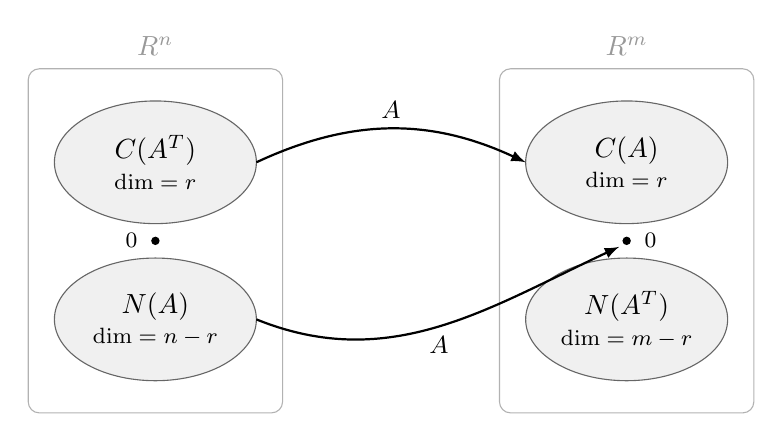
\begin{tikzpicture}[scale=0.95,>=latex]
  % --- caja izquierda: R^n ---
  \draw[rounded corners=4pt,gray!60] (-0.1,-2.3) rectangle (3.3,2.3);
  \node[gray!80] at (1.6,2.6) {$\mathbb{R}^n$};
  \draw[fill=gray!12,draw=black!60] (1.6,1.05) ellipse (1.35 and 0.82);
  \draw[fill=gray!12,draw=black!60] (1.6,-1.05) ellipse (1.35 and 0.82);
  \node[align=center] at (1.6,1.05) {$C(A^T)$\\[-1pt]{\footnotesize $\dim = r$}};
  \node[align=center] at (1.6,-1.05) {$N(A)$\\[-1pt]{\footnotesize $\dim = n-r$}};
  \fill (1.6,0) circle (1.6pt);
  \node[font=\footnotesize,left=3pt] at (1.6,0) {$\n{0}$};
  % --- caja derecha: R^m ---
  \draw[rounded corners=4pt,gray!60] (6.2,-2.3) rectangle (9.6,2.3);
  \node[gray!80] at (7.9,2.6) {$\mathbb{R}^m$};
  \draw[fill=gray!12,draw=black!60] (7.9,1.05) ellipse (1.35 and 0.82);
  \draw[fill=gray!12,draw=black!60] (7.9,-1.05) ellipse (1.35 and 0.82);
  \node[align=center] at (7.9,1.05) {$C(A)$\\[-1pt]{\footnotesize $\dim = r$}};
  \node[align=center] at (7.9,-1.05) {$N(A^T)$\\[-1pt]{\footnotesize $\dim = m-r$}};
  \fill (7.9,0) circle (1.6pt);
  \node[font=\footnotesize,right=3pt] at (7.9,0) {$\n{0}$};
  % --- flechas ---
  \draw[->,thick] (2.95,1.05) to[out=25,in=155] node[above,font=\small] {$A$} (6.55,1.05);
  \draw[->,thick] (2.95,-1.05) to[out=-22,in=205] node[below,font=\small] {$A$} (7.80,-0.08);
\end{tikzpicture}
\caption{Los cuatro subespacios fundamentales de una matriz $A$ de $m\times n$ y
rango $r$. El espacio fila se transforma sobre el espacio columna; el espacio
nulo se aplasta en el origen.}
\label{fig:cuatro-subespacios}
\end{figure}

\begin{remark}[Lo que falta de esta figura]\label{obs:ortogonalidad-pendiente}
Los cuatro subespacios no son cuatro objetos sueltos. Dentro de $\mathbb{R}^n$,
el espacio fila y el espacio nulo son \emph{perpendiculares} entre sí, y de
hecho cada uno es todo lo que le falta al otro para completar $\mathbb{R}^n$; lo
mismo ocurre en $\mathbb{R}^m$ con el espacio columna y el nulo izquierdo. Para
enunciarlo y demostrarlo con precisión necesitamos el producto interno y la
noción de complemento ortogonal, así que lo dejamos para el
Capítulo~\ref{cap:ortogonalidad}, donde probaremos que
\[
N(A) = C(A^T)^{\perp}
\qquad\text{y}\qquad
N(A^T) = C(A)^{\perp}.
\]
Por ahora nos concentramos en la otra mitad de la figura: las dimensiones.
\end{remark}

\section{Rango y la factorización $A=CR$}
\label{sec:CR}

La pregunta natural es cuál es la dimensión de cada uno de los cuatro
subespacios. Empecemos por el espacio columna: para conocer su dimensión hay que
construir una base, y para eso alcanza con recorrer las columnas de $A$
quedándonos sólo con las que aportan información nueva.

\begin{enumerate}[itemsep=1pt]
    \item Si la primera columna de $A$ no es nula, la ponemos como primera
    columna de una nueva matriz $C$ (si es nula, la descartamos y seguimos).
    \item Si la segunda columna de $A$ no es múltiplo de la primera retenida, la
    agregamos a $C$.
    \item Si la tercera no es combinación lineal de las ya retenidas, la
    agregamos a $C$.
    \item Seguimos así hasta recorrer todas las columnas de $A$.
\end{enumerate}

Al terminar, las $r$ columnas de $C \in \mathbb{R}^{m \times r}$ son
linealmente independientes por construcción y generan $C(A)$, porque las
columnas descartadas eran combinación lineal de las retenidas. Es decir, las
columnas de $C$ son una base de $C(A)$ y
\[
\dim C(A) = r .
\]

¿Cómo se relacionan $A$ y $C$? Cada columna $\n{a}_j$ de $A$ es combinación
lineal de las columnas de $C$: existen coeficientes $r_{1j},\dots,r_{rj}$ con
\[
\n{a}_j = r_{1j}\n{c}_1 + \cdots + r_{rj}\n{c}_r = C\n{r}_j,
\qquad
\n{r}_j = \begin{bmatrix} r_{1j} & \cdots & r_{rj}\end{bmatrix}^T \in\mathbb{R}^r .
\]
Poniendo estos vectores uno al lado del otro y usando \eqref{eq:cols} para
armar $R = \begin{bmatrix} \n{r}_1 & \cdots & \n{r}_n \end{bmatrix}
\in \mathbb{R}^{r \times n}$, obtenemos la \textbf{descomposición $CR$}:
\[
\boxed{\ A = CR\ },
\qquad C\in\mathbb{R}^{m\times r},\quad R\in\mathbb{R}^{r\times n}.
\]

\begin{example}\label{ej:CR}
Para $A \in \mathbb{R}^{3 \times 4}$,
\[
A = \begin{bmatrix}
    1 & 2 & 5 & 2 \\
    0 & 1 & 2 & 1 \\
    0 & 3 & 6 & 3
\end{bmatrix} =
\begin{bmatrix} 1 & 2 \\ 0 & 1 \\ 0 & 3 \end{bmatrix}
\begin{bmatrix} 1 & 0 & 1 & 0 \\ 0 & 1 & 2 & 1 \end{bmatrix} = CR .
\]
Las columnas retenidas son la $1$ y la $2$; la tercera es
$\n{a}_3 = \n{a}_1 + 2\n{a}_2$ y la cuarta es $\n{a}_4 = \n{a}_2$, y eso es
exactamente lo que dicen las columnas $3$ y $4$ de $R$.
\end{example}

Observemos una consecuencia del procedimiento: como las columnas de $C$ son
columnas de $A$, cada una de ellas se expresa a sí misma en la base $C$
mediante un vector canónico. Por lo tanto, \emph{en las posiciones de $R$
correspondientes a las columnas elegidas aparece la matriz identidad $I_r$} (en
el Ejemplo~\ref{ej:CR}, en las columnas $1$ y $2$). En particular las $r$ filas
de $R$ son linealmente independientes.

\begin{remark}[$C$ y $R$ no son únicas]
El procedimiento elige las columnas independientes de izquierda a derecha, pero
cualquier otra elección de $r$ columnas independientes de $A$ sirve igual y da
otra factorización $A=CR$. En el Ejemplo~\ref{ej:CR} podríamos haber tomado las
columnas $1$ y $4$. Esta libertad, lejos de ser un defecto, es lo que se explota
en la Sección~\ref{sec:CMR}.
\end{remark}

\begin{remark}[Cómo se calcula en la práctica]
El procedimiento de arriba es heurístico: dice qué hay que hacer, no cómo
hacerlo de manera sistemática. La eliminación gaussiana del
Capítulo~\ref{cap:LU} responde esa pregunta: las columnas retenidas son las
columnas \emph{pivote} de $A$, y $R$ resulta ser la forma escalonada reducida
por filas de $A$ sin sus filas nulas.
\end{remark}

\subsection{El rango}

La factorización $A=CR$ nos regala la dimensión del espacio fila. Trasponiendo,
\begin{equation}
A^T = R^T C^T .
\label{eq:At}
\end{equation}
Como $R$ tiene $r$ filas independientes, $R^T\in\mathbb{R}^{n\times r}$ tiene
$r$ columnas independientes, y \eqref{eq:At} dice que las columnas de $A^T$
--- o sea las filas de $A$ --- son combinación lineal de ellas. Luego las filas
de $R$ son una base del espacio fila y
\[
\dim C(A^T) = r .
\]

Este número $r$, que cuenta simultáneamente las columnas independientes y las
filas independientes de $A$, es el \textbf{rango} de $A$:
\[
\boxed{\ \dim C(A) = \dim C(A^T) = \rg(A) = r\ }
\]
Vale la pena detenerse en lo que acaba de pasar: aunque $C(A) \subseteq
\mathbb{R}^m$ y $C(A^T) \subseteq \mathbb{R}^n$ viven en espacios ambientes de
dimensiones distintas, tienen exactamente la misma dimensión interna. No hay
ninguna razón evidente para que la cantidad de columnas independientes coincida
con la de filas independientes, y sin embargo así es.

\subsection{Los espacios nulos y el teorema de la dimensión}

Con $A=CR$ también se obtienen las dimensiones de los espacios nulos, sin
invocar ningún resultado externo.

\begin{proposition}\label{prop:NA-NR}
Si $A = CR$ con $C\in\mathbb{R}^{m\times r}$ de columnas linealmente
independientes, entonces $N(A) = N(R)$.
\end{proposition}

\begin{proof}
Si $R\n{x} = \n{0}$ entonces $A\n{x} = C(R\n{x}) = \n{0}$, así que
$N(R)\subseteq N(A)$. Recíprocamente, si $A\n{x} = \n{0}$, llamando
$\n{y} = R\n{x}\in\mathbb{R}^r$ tenemos $C\n{y} = \n{0}$; pero $C\n{y}$ es la
combinación lineal de las columnas de $C$ con coeficientes $\n{y}$, y esas
columnas son independientes, de modo que $\n{y} = \n{0}$, es decir
$R\n{x} = \n{0}$.
\end{proof}

\begin{theorem}[Teorema de la dimensión]\label{teo:rango-nulidad}
Para toda $A\in\mathbb{R}^{m\times n}$ de rango $r$,
\[
\rg(A) + \dim N(A) = n,
\qquad\text{esto es}\qquad
\dim N(A) = n-r .
\]
\end{theorem}

\begin{proof}
Por la Proposición~\ref{prop:NA-NR} alcanza con calcular $\dim N(R)$.
Reordenando las columnas de $A$ (lo que sólo reordena las de $R$ y no cambia
dimensiones) podemos suponer que las columnas elegidas para $C$ son las primeras
$r$, de modo que $R = \begin{bmatrix} I_r & R_2\end{bmatrix}$ con
$R_2\in\mathbb{R}^{r\times(n-r)}$. Partiendo
$\n{x} = \begin{bsmallmatrix}\n{x}_1\\ \n{x}_2\end{bsmallmatrix}$ con
$\n{x}_1\in\mathbb{R}^r$ y $\n{x}_2\in\mathbb{R}^{n-r}$,
\[
R\n{x} = \n{x}_1 + R_2\n{x}_2 = \n{0}
\iff
\n{x}_1 = -R_2\n{x}_2 .
\]
Es decir, $\n{x}_2$ es libre y $\n{x}_1$ queda determinado: la aplicación
$\n{x}_2 \mapsto \begin{bsmallmatrix}-R_2\n{x}_2\\ \n{x}_2\end{bsmallmatrix}$ es
un isomorfismo de $\mathbb{R}^{n-r}$ sobre $N(R)$. Luego
$\dim N(A) = \dim N(R) = n-r$.
\end{proof}

Aplicando el mismo teorema a $A^T\in\mathbb{R}^{n\times m}$, cuyo espacio de
partida es $\mathbb{R}^m$ y cuyo rango también es $r$, obtenemos
$\dim N(A^T) = m-r$. Las cuatro dimensiones quedan entonces determinadas por
tres números, $m$, $n$ y $r$:

\[
\begin{array}{l|c|c}
\text{Subespacio} & \text{vive en} & \text{dimensión} \\
\hline
\text{Espacio columna } C(A) & \mathbb{R}^m & r \\[0.5ex]
\text{Espacio fila } C(A^T) & \mathbb{R}^n & r \\[0.5ex]
\text{Espacio nulo } N(A) & \mathbb{R}^n & n - r \\[0.5ex]
\text{Espacio nulo izquierdo } N(A^T) & \mathbb{R}^m & m - r
\end{array}
\]

\begin{entrega}{El rango de un producto y de una suma}\label{ent:rango}
Las desigualdades que siguen se usan en todo el apunte, casi siempre sin
mencionarlas. Todas salen de mirar espacios columna; ninguna necesita
coordenadas. En todos los ítems $A$ y $B$ tienen los tamaños que hacen falta
para que las operaciones tengan sentido.

\begin{enumerate}[label=\textbf{(\alph*)},itemsep=3pt,topsep=4pt]
\item Probar que $C(AB) \subseteq C(A)$ y que $C\big((AB)^T\big) \subseteq C(B^T)$.
Deducir que
\[
\rg(AB) \le \min\{\rg(A),\, \rg(B)\}.
\]
Dar un ejemplo de matrices no nulas $A,B$ con $AB=0$.

\item Probar que si $B$ es invertible entonces $\rg(AB) = \rg(A)$, y que si $A$
es invertible entonces $\rg(AB)=\rg(B)$. \emph{Multiplicar por matrices
invertibles no cambia el rango}: esto es lo que hace que la eliminación
gaussiana, la semejanza y la SVD conserven el rango.

\item Probar que $C(A+B) \subseteq C(A) + C(B)$ y deducir que
\[
\rg(A+B) \le \rg(A) + \rg(B).
\]
Dar un ejemplo donde valga la igualdad y otro donde la desigualdad sea estricta.

\item Probar que $N(A^TA) = N(A)$ y concluir que $\rg(A^TA) = \rg(A)$.
\emph{Sugerencia:} si $A^TA\n{x} = \n{0}$, multiplicar por $\n{x}^T$ y reconocer
$\|A\n{x}\|^2$.

\item Probar que $\rg(A) = r$ si y sólo si $A$ se puede escribir como suma de
$r$ matrices de rango $1$, y no de menos. \emph{Sugerencia:} para una
implicación usar \eqref{eq:suma-rango1} aplicada a $A=CR$; para la otra, el
ítem (c).

\item \emph{(Desigualdad de Sylvester --- opcional.)} Sean
$A\in\mathbb{R}^{m\times n}$ y $B\in\mathbb{R}^{n\times p}$. Probar que
\[
\dim N(AB) \;=\; \dim N(B) \;+\; \dim\big(C(B)\cap N(A)\big)
\]
y deducir, usando el Teorema~\ref{teo:rango-nulidad}, que
\[
\rg(AB) \ \ge\ \rg(A) + \rg(B) - n .
\]
Verificar la fórmula en un ejemplo de $2\times2$ en el que la cota se alcance.
\end{enumerate}

\medskip
\noindent{\footnotesize\emph{Se entrega por escrito. Los ítems (b), (d) y (e) se
usan en los capítulos de ortogonalidad, de matrices simétricas y de la SVD
respectivamente. El ítem (f) es opcional.}}
\end{entrega}

\section[La factorización $A=CMR$]{Columnas y filas de verdad: $A=CMR$}
\label{sec:CMR}

La descomposición $A=CR$ tiene una asimetría que conviene mirar de cerca. Las
columnas de $C$ son columnas \emph{de $A$}: son datos originales. Las filas de
$R$, en cambio, no son filas de $A$; son los coeficientes que reconstruyen $A$ a
partir de $C$. En el Ejemplo~\ref{ej:CR} las filas de $R$ son $(1,0,1,0)$ y
$(0,1,2,1)$, que no aparecen en ningún lado de $A$.

Cuando la matriz viene de datos, esa asimetría importa. Si las columnas de $A$
son pacientes y las filas son genes, uno quisiera que \emph{ambos} factores
estén hechos de pacientes y de genes reales, no de combinaciones lineales
abstractas de ellos. Esa es la idea de la factorización
\[
A = C\,M\,\n{R},
\]
donde $C$ contiene $r$ columnas de $A$, $\n{R}$ contiene $r$ filas de $A$, y la
matriz invertible $M\in\mathbb{R}^{r\times r}$, llamada \textbf{matriz de
mezcla}, es la que hace que la igualdad sea cierta. Las factorizaciones $QR$ y
la SVD, que veremos más adelante, son numéricamente mucho mejores pero pagan un
precio: sus factores están formados por vectores ortogonalizados, que ya no son
datos.

\begin{entrega}{La factorización $A=CMR$}
Sea $A\in\mathbb{R}^{m\times n}$ de rango $r$. Sea $C\in\mathbb{R}^{m\times r}$
una matriz formada por $r$ columnas linealmente independientes de $A$ y sea
$\n{R}\in\mathbb{R}^{r\times n}$ una matriz formada por $r$ filas linealmente
independientes de $A$.

\begin{enumerate}[label=\textbf{(\alph*)},itemsep=3pt,topsep=4pt]
\item Probar que $C^TC$ y $\n{R}\n{R}^T$ son invertibles. \emph{Sugerencia:} son
de $r\times r$ y se puede usar el ítem (d) de la entrega anterior.

\item \emph{(Existencia.)} Sea $A=CR$ la factorización de la
Sección~\ref{sec:CR}. Justificar que las filas de $R$ pertenecen al espacio fila
de $A$ y que las filas de $\n{R}$ son una base de ese espacio. Deducir que
existe $M\in\mathbb{R}^{r\times r}$ con $R = M\n{R}$, y por lo tanto
\[
A = C\,M\,\n{R}.
\]
Probar además que $M$ es invertible.

\item \emph{(Fórmula.)} Partiendo de $A = CM\n{R}$, multiplicar por $C^T$ a
izquierda y por $\n{R}^T$ a derecha y despejar
\[
M = (C^TC)^{-1}\,\big(C^T A\,\n{R}^T\big)\,(\n{R}\,\n{R}^T)^{-1}.
\tag{$*$}
\]
Concluir que $M$ es única.

\item \emph{(Rango 1.)} Verificar con $(*)$ que para
$A = \begin{bsmallmatrix} 2 & 4\\ 3& 6\end{bsmallmatrix}$, tomando la primera
columna y la primera fila, se obtiene $M = \begin{bsmallmatrix}
\tfrac12\end{bsmallmatrix}$. Probar en general que si $A = \n{u}\n{v}^T$ es de
rango $1$ y se eligen la columna $j$ y la fila $i$ con $a_{ij}\neq 0$, entonces
$M = \begin{bsmallmatrix} 1/a_{ij}\end{bsmallmatrix}$.

\item \emph{(Un caso de rango 2.)} Para
\[
A = \begin{bmatrix} 1 & 3 & 8\\ 1& 2& 6\\ 0&1&2\end{bmatrix},
\]
tomar $C$ con las columnas $1$ y $2$ y $\n{R}$ con las filas $1$ y $2$. Calcular
$M$ con la fórmula $(*)$ y verificar que $A = CM\n{R}$.

\item \emph{(Lo que la fórmula esconde.)} Sean $I=\{i_1,\dots,i_r\}$ las filas
de $A$ elegidas para $\n{R}$ y $J=\{j_1,\dots,j_r\}$ las columnas elegidas para
$C$, y sea $W\in\mathbb{R}^{r\times r}$ la submatriz de $A$ que queda en el
cruce de esas filas y columnas. Probar que
\[
M = W^{-1}.
\]
\emph{Sugerencia:} quedarse con las filas $I$ de los dos miembros de
$A = CM\n{R}$ y observar qué matriz es la formada por las filas $I$ de $\n{R}$.
Verificarlo en el ítem (e). Discutir, a partir de esto, por qué al elegir las
filas y columnas conviene que $W$ esté lo más lejos posible de ser singular.

\end{enumerate}

\medskip
\noindent{\footnotesize\emph{Se entrega por escrito. El ítem (f) explica por qué
esta factorización, bajo el nombre de descomposición \textnormal{CUR}, se usa
hoy para matrices grandes.}}
\end{entrega}

\section{Actualizaciones de rango uno}
\label{sec:rango-uno}

Cerramos el capítulo con una última aparición del producto externo, esta vez en
un papel distinto. En muchas aplicaciones no se resuelve un problema una sola
vez: se resuelve, llega un dato nuevo, y hay que volver a resolverlo con una
matriz que difiere de la anterior en muy poco. Si ese ``muy poco'' es una matriz
de rango $1$ --- agregar una observación, corregir una entrada, quitar un dato
del conjunto ---, entonces no hace falta empezar de cero: la inversa se puede
\emph{actualizar}. La fórmula que hace eso se conoce como fórmula de
Sherman--Morrison, y es sorprendentemente simple.

\begin{entrega}{Actualizaciones de rango uno: Sherman--Morrison}\label{ent:sherman}
Sea $A\in\mathbb{R}^{n\times n}$ invertible y sean $\n{u},\n{v}\in\mathbb{R}^n$.

\begin{enumerate}[label=\textbf{(\alph*)},itemsep=3pt,topsep=4pt]
\item Supongamos $1+\n{v}^TA^{-1}\n{u}\neq0$. Verificar, multiplicando
directamente, que
\[
\big(A+\n{u}\n{v}^T\big)^{-1}
= A^{-1} - \frac{A^{-1}\n{u}\,\n{v}^TA^{-1}}{1+\n{v}^TA^{-1}\n{u}} .
\]
\emph{Sugerencia:} el único truco es notar que $\n{v}^TA^{-1}\n{u}$ es un
\emph{número}, y que por lo tanto se puede mover libremente dentro del producto.

\item Probar el recíproco: si $1+\n{v}^TA^{-1}\n{u}=0$, entonces
$A+\n{u}\n{v}^T$ es singular. \emph{Sugerencia:} exhibir un vector no nulo del
espacio nulo usando $A^{-1}\n{u}$.

\item Contar operaciones: suponiendo que ya se conoce $A^{-1}$, ¿cuántas
operaciones cuesta aplicar la fórmula del ítem (a)? Invertir
$A+\n{u}\n{v}^T$ desde cero cuesta del orden de $n^3$ operaciones.

\item Probar que $\rg(A+\n{u}\n{v}^T)$ y $\rg(A)$ difieren en a lo sumo $1$
(usar el ítem (c) del Ejercicio de desarrollo~\ref{ent:rango}). Dar ejemplos de
los tres casos posibles: que el rango suba, que baje, y que no cambie.

\item \emph{(Para pensar, sin cuentas.)} En un modelo lineal se trabaja con la
matriz $A = X^TX$, donde cada fila de $X$ es una observación. Si se quita una
observación $\n{x}_i$, la nueva matriz es $A - \n{x}_i\n{x}_i^T$. Explicar por
qué los ítems anteriores permiten recalcular el modelo sin la observación $i$
para cada $i$, a un costo mucho menor que rehacer todo $n$ veces.
\end{enumerate}

\medskip
\noindent{\footnotesize\emph{Se entrega por escrito. El ítem (e) es la base de
la validación cruzada \textnormal{leave-one-out}; la fórmula del ítem (a)
reaparece cada vez que hay que actualizar un modelo con datos nuevos.}}
\end{entrega}

\section{Resumen de notación}

A lo largo del apunte usaremos sistemáticamente lo siguiente.

\begingroup
\medskip
\centering
\small
\setlength{\tabcolsep}{5pt}
\renewcommand{\arraystretch}{1.0}
\begin{tabular}{@{}ll@{}}
\hline
$\n{x},\n{y},\n{v}$ & vectores columna; $\n{x}^T$ es un vector fila \\
$\n{e}_i$ & $i$-ésimo vector de la base canónica \\
$\n{0}$ & vector nulo (o matriz nula, según el contexto) \\
$A,B,C$ & matrices; $a_{ij}=(A)_{ij}$ \\
$\fila_i(A),\ \col_j(A)$ & fila $i$ y columna $j$ de $A$ \\
$A^T$ & traspuesta; $A^{-1}$, inversa \\
$I$, $I_n$ & matriz identidad \\
$\diag(d_1,\dots,d_n)$ & matriz diagonal \\
$\langle \n{x},\n{y}\rangle = \n{x}^T\n{y}$ & producto escalar usual en $\mathbb{R}^n$ \\
$\n{x}\otimes\n{y} = \n{x}\n{y}^T$ & producto externo (matriz de rango $\le 1$) \\
$\gen(S)$ & subespacio generado por $S$ \\
$C(A)=\im(A)$ & espacio columna \\
$N(A)=\ker(A)$ & espacio nulo \\
$C(A^T)$, $N(A^T)$ & espacio fila y espacio nulo izquierdo \\
$\rg(A)$ & rango \\
$\tr(A)$ & traza \\
$\langle A,B\rangle_F=\tr(A^TB)$, $\|A\|_F$ & producto interno y norma de Frobenius \\
$\dim V$ & dimensión \\
$U\oplus W$, $V^{\perp}$ & suma directa, complemento ortogonal (Cap.~\ref{cap:ortogonalidad}) \\
\hline
\end{tabular}
\par
\endgroup

\section*{Ejercicios}

\begin{enumerate}[leftmargin=*,label=\textbf{1.\arabic*}]
\item Sean $\n{u} \in \mathbb{R}^m$ y $\n{v} \in \mathbb{R}^n$ dos vectores columna no nulos. Definimos la matriz $M = \n{u}\n{v}^T \in \mathbb{R}^{m \times n}$.
\begin{enumerate}[label=\alph*)]
    \item ¿Qué dirección tiene siempre el vector resultante $M\n{x}$ para cualquier $\n{x} \in \mathbb{R}^n$?
    \item Deduzca a partir de lo anterior cuál es el espacio columna $C(M)$ y cuál es el espacio nulo $N(M)$.
\end{enumerate}

\item Considere la matriz
\[
M = \begin{bmatrix} 2 & -4 & 6 \\ 1 & -2 & 3 \\ -3 & 6 & -9 \end{bmatrix}.
\]
\begin{enumerate}[label=\alph*)]
    \item Encuentre dos vectores $\n{x}, \n{y} \in \mathbb{R}^3$ tales que $M = \n{x} \otimes \n{y} = \n{x}\n{y}^T$.
    \item Sin calcular $N(M)$ mediante eliminación gaussiana, argumente geométricamente por qué la imagen de esta matriz es una recta y halle la ecuación del plano que define a su espacio nulo $N(M)$.
\end{enumerate}

\item Sean $\n{c}_1, \n{c}_2, \n{c}_3 \in \mathbb{R}^m$ las tres columnas de una matriz $A \in \mathbb{R}^{m \times 3}$. Suponga que no conoce los elementos individuales de $A$, pero sabe que sus columnas son vectores no nulos.
\begin{enumerate}[label=\alph*)]
    \item Exprese mediante un producto matriz-vector de la forma $A\n{x}$ el vector de salida $\n{y} \in \mathbb{R}^m$ que resulta de realizar las siguientes operaciones:
    \begin{enumerate}[label=\roman*)]
        \item Restar la segunda columna de la primera.
        \item Calcular el promedio de las tres columnas.
        \item Duplicar la primera columna y anular la tercera.
    \end{enumerate}
    \item Si se sabe que las columnas de $A$ satisfacen la relación lineal $\n{c}_3 = 2\n{c}_1 - \n{c}_2$, encuentre un vector no nulo $\n{x} \in \mathbb{R}^3$ tal que $A\n{x} = \n{0}$, sin calcular componentes individuales.
\end{enumerate}

\item Dada una matriz arbitraria $X \in \mathbb{R}^{4 \times n}$, cuyas filas denotamos por $\n{f}_1, \n{f}_2, \n{f}_3, \n{f}_4 \in \mathbb{R}^{1 \times n}$, y sin realizar multiplicaciones componente a componente, construya la matriz $E \in \mathbb{R}^{4 \times 4}$ tal que el producto $EX$ produzca una nueva matriz cuyas filas sean:
\begin{enumerate}[label=\alph*)]
    \item la primera fila multiplicada por $2$;
    \item la segunda y la tercera fila intercambiadas entre sí;
    \item la cuarta fila reemplazada por la diferencia $\n{f}_4 - \n{f}_1$.
\end{enumerate}

\item Considere las matrices $A \in \mathbb{R}^{3 \times 2}$ y $B \in \mathbb{R}^{2 \times n}$, expresadas en función de sus columnas y filas respectivamente:
\[
A = \begin{bmatrix} 1 & 0 \\ 2 & 1 \\ 0 & -1 \end{bmatrix}, \quad
B = \begin{bmatrix} \n{b}_1 \\ \n{b}_2 \end{bmatrix},
\]
donde $\n{b}_1, \n{b}_2 \in \mathbb{R}^{1 \times n}$ son los dos renglones de $B$.
\begin{enumerate}[label=\alph*)]
    \item Escriba el producto $AB \in \mathbb{R}^{3 \times n}$ como la suma de dos matrices de rango $1$ utilizando el producto externo.
    \item Si la segunda fila de $B$ es nula, determine el rango de $AB$ (asumiendo $\n{b}_1 \neq \n{0}$).
\end{enumerate}

\item Sea $A \in \mathbb{R}^{m \times n}$ de rango $r$, cuya descomposición $CR$ adopta la forma
\[
A = C \begin{bmatrix} I_r & R_2 \end{bmatrix},
\]
con $C \in \mathbb{R}^{m \times r}$ y $R_2 \in \mathbb{R}^{r \times (n-r)}$.
\begin{enumerate}[label=\alph*)]
    \item Particionando $A = \begin{bmatrix} A_1 & A_2 \end{bmatrix}$, con $A_1 \in \mathbb{R}^{m \times r}$ y $A_2 \in \mathbb{R}^{m \times (n-r)}$, efectúe la multiplicación por bloques.
    \item Deduzca la relación exacta entre $A_1$ y $C$.
    \item Exprese $A_2$ en términos de $C$ y $R_2$.
\end{enumerate}

\item Considere la matriz
\[
A = \begin{bmatrix} 1 & 3 & 2 & 0 \\ 2 & 6 & 4 & 1 \\ 0 & 0 & 0 & 2 \end{bmatrix} \in\mathbb{R}^{3\times 4}.
\]
\begin{enumerate}[label=\alph*)]
    \item Aplique el procedimiento de la Sección~\ref{sec:CR} para obtener la matriz $C$.
    \item Deduzca $R$ resolviendo $A = CR$ columna por columna, interpretando cada columna de $R$ como las coordenadas de la columna correspondiente de $A$ en la base $C$.
    \item Verifique que $I_r$ aparece incrustada en las columnas correspondientes de $R$.
\end{enumerate}

\item Sea $A \in \mathbb{R}^{m \times n}$ de rango $r$.
\begin{enumerate}[label=\alph*)]
    \item Considere $B = \begin{bmatrix} A & A \end{bmatrix} \in \mathbb{R}^{m \times 2n}$. Exprese $B\n{x}$ por bloques para $\n{x} = \begin{bsmallmatrix} \n{x}_1 \\ \n{x}_2 \end{bsmallmatrix}$ y determine $\rg(B)$, $C(B)$ y $\dim N(B)$.
    \item Considere ahora $D = \begin{bsmallmatrix} A \\ A \end{bsmallmatrix} \in \mathbb{R}^{2m \times n}$ y determine $\rg(D)$, $C(D)$ y $\dim N(D)$.
\end{enumerate}

\item\label{ej:traza} Sean $A \in \mathbb{R}^{m\times n}$ y $B\in\mathbb{R}^{n\times m}$.
\begin{enumerate}[label=\alph*)]
    \item Probar que $\tr(AB) = \tr(BA)$, escribiendo ambos miembros como una doble suma.
    \item Dar un ejemplo con $\tr(AB)=\tr(BA)$ pero $AB \neq BA$.
    \item Probar que $\tr(\n{x}\n{y}^T) = \n{y}^T\n{x}$ para $\n{x},\n{y}\in\mathbb{R}^n$.
\end{enumerate}

\item Dada una matriz cuadrada $P \in \mathbb{R}^{n \times n}$ que cumple $P^2 = P$ (se dice que $P$ es \emph{idempotente}):
\begin{enumerate}[label=\alph*)]
    \item Muestre que si $\n{y} \in C(P)$, entonces $P\n{y} = \n{y}$.
    \item Demuestre que cualquier $\n{x} \in \mathbb{R}^n$ se descompone de forma única como
    \[
    \n{x} = P\n{x} + (I - P)\n{x},
    \]
    donde $P\n{x} \in C(P)$ y $(I - P)\n{x} \in N(P)$. Es decir,
    $\mathbb{R}^n = C(P)\oplus N(P)$.
    \item Usando el Ejercicio~\ref{ej:traza}, ¿qué relación sospecha entre
    $\tr(P)$ y $\rg(P)$? (La probaremos en el Capítulo~\ref{cap:autovalores}.)
\end{enumerate}
\end{enumerate}
